
\section{Le unità di misura della Fisica Nucleare e Subnucleare}
\label{sec:unita-di-misura}

La scelta della unità di misura è arbitraria ma, in accordo con i criteri che ispirano i moderni sistemi, soddisfa
alcuni semplici requisiti di ordine generale:
\begin{itemize}
    \item  \textbf{l'unità deve essere connessa ad un fenomeno naturale ritenuto stabile ed invariabile nel tempo} piuttosto che ad un oggetto o manufatto particolare il quale potrebbe deteriorarsi o modificare le sue proprietà con il tempo;
    \item  \textbf{le unità non devono essere ridondanti} e devono costituire un sistema di grandezze fisiche irriducibili dette fondamentali dalle quali ottenere tutte le altre che invece vengono dette derivate;
    \item  \textbf{l'unità deve essere riproducibile in laboratorio con una relativa facilità} (in realtà è lavoro da professionisti quali sono i metrologi).
\end{itemize}

Un sistema di unità di misura più appropriato può essere costruito facendo riferimento alle costanti fisiche fondamentali che governano i fenomeni nucleari e subnucleari.
Accanto alle grandezze fondamentali, ogni area della fisica introduce anche specifiche costanti fisiche.
Queste possono essere sia dimensionali che adimensionali, riferirsi a specifiche classi di fenomeni - e dunque di rango locale - oppure valide per ogni fenomeno fisico e quindi di rango universale.

Mentre il valore numerico delle costanti dimensionali dipende dalla scelta del sistema di unità misura, quello delle
costanti adimensionali ne è del tutto indipendente per cui si ritiene che siano dotate di un più profondo significato
fisico anche se a tutt’oggi nessuna teoria è in grado di predirne il valore.
Fu Planck che propose di assumere come grandezze fisiche fondamentali le costanti fisiche universali introducendo i
cosiddetti sistemi naturali di unità di misura.
Lo scopo di tali sistemi è quello di dedurre le appropriate scale di lunghezze, tempi, masse e temperature direttamente
dai fenomeni naturali piuttosto che da convenzioni di natura metrologica.

La costruzione di un sistema di unità di misura le cui grandezze abbiano la scala appropriata pxer una certa classe di
fenomeni richiede l'introduzione di specifici vincoli tra le grandezze fondamentali della descrizione macroscopica.
Ad esempio, dato che \textbf{i fenomeni nucleari e subnucleari sono al tempo stesso relativistici e quantistici} ciò
significa che le velocità, ovvero i quozienti tra lunghezze e tempi saranno dell'ordine di c, mentre le azioni, cioè i
prodotti delle energie per i tempi caratteristici saranno dell'ordine di $\hslash$.
Due costanti universali non sono però sufficienti per fissare la scala delle tre grandezze necessarie al Sistema
Internazionale per descrivere la relatività e meccanica quantistica (L, T ed M).
Il particolare ruolo giocato dalle macchine acceleratrici in fisica nucleare e delle particelle elementari suggerisce
allora di assumere come terza grandezza (non costante) un fondamentale parametro costruttivo della macchina, \textbf{l'energia E}.
In accordo con le convenzioni adottate nella ingegneria delle macchine acceleratrici si assume come unità l'elettronvolt
(eV), ovvero l'energia cinetica acquisita da un elettrone accelerato da una differenza di potenziale di un volt.
Si ottiene facilmente la sua conversione in joule: $E_\text{cin} = eV$ da cui $1 eV = 1.602 \times 10^{-19} \ J$.

Definite le unità del \textbf{Sistema Naturale della Fisica Nucleare e Subnucleare (SNNS)} possiamo facilmente calcolare
i loro valori nel Sistema Internazionale (SI) attraverso le seguenti equazioni dimensionali (si noti che con le lettere
minuscole indichiamo le grandezze fondamentali del SNNS e con le maiuscole quelle del SI)
\begin{gather*}
    c \sim \frac{L}{T} \qquad \epsilon \sim M c^2 \qquad \epsilon T \sim \hslash\\
    L \sim cT \qquad M \sim \frac{\epsilon}{c^2} \qquad T \sim \frac{\hslash}{\epsilon} \\
     L \sim \frac{\hslash c}{\epsilon} \qquad M \sim \frac{\epsilon}{c^2} \qquad T \sim  \frac{\hslash}{\epsilon}\\
\end{gather*}
Da queste deduciamo che le lunghezze possono essere misurate in unità di $\frac{\hslash c}{\epsilon}$ ($\hslash c / eV$ o $1/eV$ se $\hslash=c=1$),
i tempi in unità di $\frac{\hslash}{\epsilon}$ ($\hslash/eV$ o $1/eV$ se $\hslash=1$) ed infine le masse in unità di $\epsilon/c^2(eV/c^2$ o $eV$ se $c=1$).

Tenendo ora presenti i valori delle costanti universali espresse nel Sistema Internazionale e della conversione tra Joule
($J$) ed elettronvolt ($eV$):
\begin{gather*}
    \hslash = 1.055 \times 10^{-34} J \cdot s \quad c = 2.998 \times 10^8 m/s \quad \hslash c = 3.162 \times 10^{-26} J \cdot m\\
    \qquad \quad 1 eV = 1.602 \times 10^{-19} J\\
\end{gather*}
possiamo calcolare i coefficienti della conversione tra il Sistema Naturale della Fisica Nucleare e Subnucleare ed il Sistema Internazionale (per quanto riguarda l'energia, piuttosto che gli eV, assumeremo la scala più appropriata dei MeV) \begin{gather*}
    L \sim \frac{\hslash c}{\epsilon} \qquad 1 \left(\frac{\hslash c}{MeV}\right) \sim 1.97      \times 10^{-19} m\\
    M \sim \frac{\epsilon}{c^2} \qquad 1 \left(\frac{MeV}{c^2}\right) \sim 1.78 \times 10^{-30} Kg\\
    \frac{\hp}{\epsilon} \sim T \qquad 1 \left ( \frac{\hp}{MeV} \right) \sim 6.59 \times 10^{-22} s\\
\end{gather*}

\section{Le proprietà generali dei nuclei}
\label{sec:proprieta-generali-dei-nuclei}

Il \textbf{nucleo} è un sistema composto formato da \textbf{neutroni} e \textbf{protoni} - spesso indicati con il nome
generico di \textbf{nucleoni} - tenuti assieme dalla \textbf{interazione forte}, una delle interazioni fondamentali
della natura(di cui non si ha traccia macroscopicamente).

In fisica nucleare si usa il termine `nuclide' piuttosto che `nucleo' più prossimo alla chimica.
Si hanno le seguenti grandezze rilevanti:
\begin{itemize}
    \item \textbf{numero atomico} $Z$, ovvero numero di protoni del nuclide;
    \item il numero di neutroni non ha nome specifico e si indica con $N$;
    \item \textbf{numero di massa} $A$, ovvero il numero di nucleoni $Z+N$.
\end{itemize}

Ne consegue che una qualunque coppia dei numeri $Z, N$ ed $A$ identifica univocamente il nuclide.
La notazione è la seguente:
\[
\mathlarger{\mathlarger{^A _{Z} X}}_N
\]

Si parla di nuclidi

\begin{enumerate}
    \item \textbf{isotopi} se hanno stesso $Z$ ma diversi $N$ ed $A$;
    \item  \textbf{isotoni} se hanno stesso $N$ ma diversi $Z$ ed $A$;
    \item \textbf{isobari} se hanno stesso $A$ ma diversi $N$ ed $Z$;
    \begin{itemize}
        \item  se questi hanno $N$ e $Z$ scambiati si dicono \emph{speculari};
    \end{itemize}
    \item \textbf{isomeri} se sono identici ma in uno stato di energia differente.
\end{enumerate}

Il neutrone ha una massa di $939.56 MeV/c^2$ che eccede di soli $1.29 MeV / c^2$ la massa del protone che ammonta a
$938.27 MeV/c^2$.
Spesso approssimate a $940 MeV/c^2$ o addirittura ad $1 GeV/c^2$, i nucleoni risultano circa $1840$ volte più massivi
dell'elettrone ($0.51 MeV/c^2$).
La piccola differenza di massa gioca un ruolo chiave in molti fenomeni.
%%TODO valuta se referenziare a possibile sezione su delta m  % (vedi \ref{sec:la-differenza-di-massa-tra-neutrone-e-protone}).
Sia i \textbf{neutroni} che i protoni possiedono un momento angolare intrinseco di \textbf{spin} $s=\frac{1}{2}$ (in unità $\hp$).
Sulla base della meccanica quantistica, ciò significa che la proiezione del momento angolare lungo un certo asse può assumere i due soli valori $\frac{1}{2} \hp$ e $-\frac{1}{2}\hp$.
Lo spin interviene non solo negli aspetti specifici della dinamica dei nucleoni ma anche nella determinazione del loro \textbf{comportamento collettivo}.
La meccanica quantistica impone ai sistemi di particelle identiche restrizioni peculiari che non hanno analogie nella fisica classica.
Sulla base del \textbf{teorema di spin statistica} i neutroni ed i protoni nucleari - che hanno spin semintero -
si comportano collettivamente come \textbf{fermioni} e devono soddisfare il \textbf{principio di Pauli}, un fatto che
gioca un ruolo decisivo nella \textbf{stabilità} e \textbf{struttura} del nucleo.

\marginnote{Momento di dipolo magnetico dei nucleoni}


Nella fisica classica solo una particella estesa può possedere momento angolare intrinseco (spin).
Se lo possiede ed è elettricamente carica allora possiede anche momento di dipolo magnetico.
Ad esempio è facile mostrare che un anello di carica $e$ e superficie $S$, posto in rotazione attorno all'asse di
simmetria, soddisfa la seguente relazione $\mu = \frac{eL}{2m}$.

Nella fisica quantistica, non solo le particelle estese (composte) ma \textbf{anche quelle puntiformi}  (elementari)
possono essere dotate di \textbf{spin} per cui - se dotate di carica elettrica - possiederanno anche un \textbf{momento di dipolo magnetico}.

Vediamo da un conto esplicito che l'analogia classica-quantistica è fallimentare:
\begin{gather*}
    \mu = i S = \frac{e}{T}\pi R^2 \\
    L = mvR = m \frac{2 \pi R}{T}R \rightarrow  \pi R^2 = \frac{T}{2m}L\\
     \rightarrow \mu = \frac{e}{T}\frac{T}{2m}L = \frac{e \hp}{2m}\left( \frac{L}{\hp}\right)
\end{gather*}
dove la grandezza $\frac{e \hp}{2m}$ viene detta \textbf{magnetone di Bohr} e vale $9.274\times 10^{-24}J/T$.
E' un fatto ben noto però che la relazione tra $\mu$ ed $L$ differisce da quella classica per un fattore numerico.
Ad esempio, nel caso di particelle puntiformi di spin $1/2$, l'equazione \textbf{quantomeccanica relativistica di Dirac}
conduce ad una relazione contenente un fattore $g$:
\[
    \mu_{qm} = g \frac{e \hp}{2m}\left( \frac{L}{\hp}\right)
\]
di valore $2$.

Preso atto di questo fatto dobbiamo aggiungere che le teorie di campo quantizzato hanno dimostrato che il fattore $g=2$
delle particelle puntiformi deve subire \textbf{piccole correzioni} dovute a certi processi virtuali, soprattutto di natura elettromagnetica, di cui diremo
\[
g = 2(1+a) \qquad a = \frac{g -2}{2}
\]
La correzione $a$ - detta \emph{momento magnetico anomalo} o anche $\frac{g -2}{2}$ - rappresenta uno dei parametri più importanti per un confronto di alta precisione tra previsioni teoriche e misure sperimentali.
A titolo di esempio nel caso dell'elettrone si ha
\begin{gather*}
    a_{th} = 0.001 159 652 181 643 (764)\\
    a_{ex} = 0.001 159 652 180 730 (280)
\end{gather*}
lo stupefacente accordo costituisce uno dei test più significativi a favore della \caps{QED}.
Nel caso in cui la particella quantistica non sia puntiforme il fattore $g=2$ si modifica ben più pesantemente.
Ad esempio, nel caso del protone deve essere moltiplicato per $2.79$ per cui si ha $g=2 \times 2.79=5.58$ mentre nel caso
del neutrone deve essere moltiplicato per $-1.91$ per cui si ha $g=2 \times(-1.91) = -3.82$.

Alcuni fatti rilevanti:
\begin{itemize}
    \item La natura dei nucleoni \emph{non è quella di particelle elementari}.
    Questo si intuisce dalla deviazione di $ g $ dal valore 2.
    Inoltre il modello a quark degli adroni conferma questo aspetto, asserendo che, in prima approssimazione, i
    nucleoni sono pensabili come \textbf{stati legati di tre quark} con `carica forte' complessiva nulla
    nello stato di minima energia.
    \item nucleoni non possiedono momento di dipolo elettrico, un fatto che ha importanti implicazioni.
    \item La strong force ha carattere attrattivo e short range;
    \item Le dimensioni lineari del nucleo sono circa $ {10}^{5} $ volte inferiori a quelle dell'atomo.
    La descrizione quantistica dei fenomeni risulta essenziale(energia a livelli discreti \ldots);
    \item Dal principio di esclusione di Pauli si hanno vincoli sulla presenza di nucleoni (1 nucleone e 1 protone al
    al massimo in ciascun quantum state) $ \rightarrow $ degenerazione dei livelli energetici;
    \item I nuclidi più stabili tenderanno ad avere un numero di neutroni un po' piu alto di quello dei protoni
    (condizione di minima energia).
\end{itemize}

Discutiamo la \textbf{stabilità} del nucleo.

\noindent Il neutrone è intrinsecamente \textbf{instabile}: può \emph{decadere}, mediamente ogni 14.8 minuti, in protone, elettrone
e  antineutrino attraverso un processo mediato dalla interazione debole detto \textbf{decadimento beta}:
\[
   n \to p + {e}^{-} + \bar{\nu}_e
\]
A ciò si aggiunge il fatto che il protone - stabile quando libero - quando fornito di sufficiente energia può dare luogo
al \textbf{decadimento beta inverso} trasformandosi in neutrone, positrone e neutrino:
\[
 p \to n + {e}^{+} + \nu_e
\]
Cerchiamo di capire se e quando tali processi possano avvenire all'interno del nucleo.

Quando un nuclide è legato nello stato stabile di minima energia dalla interazione forte, accade che le interazioni
deboli siano bloccate dal principio di Pauli(\textbf{Pauli blocking}
\sidenote{
A causa del principio di Pauli, quando il nuclide si trova nello stato stabile di minima energia, i livelli 
energetici discretizzati dei protoni e dei neutroni sono riempiti dal basso verso l’alto occupando tutti gli stati 
quantici disponibili.
In questa situazione la trasformazione di un neutrone in protone può risultare energeticamente impossibile poiché può 
accadere che il protone finale non abbia sufficiente energia per occupare il primo stato quantico disponibile. 

A maggior ragione può risultare energeticamente impossibile la trasformazione di un protone in neutrone già penalizzata
dalla differenza di massa negativa.}\label{sn:pauli-blocking}) per cui i nucleoni diventano stabili rispetto al
decadimento beta e beta inverso.
\begin{marginfigure}
    \centering
    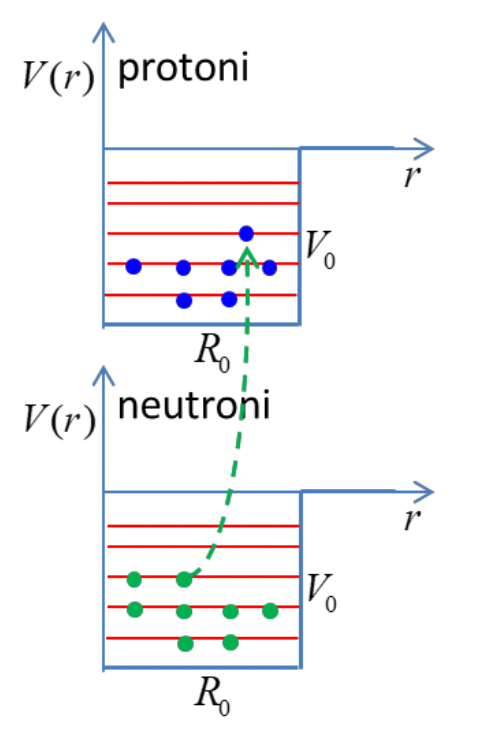
\includegraphics{figs/pauli-blocking}
%        \caption{}
    \label{fig:pauli-blocking}
\end{marginfigure}

Naturalmente, le precedenti considerazioni non valgono quando il nucleo si trova al di fuori della condizione di
equilibrio a causa di un eccesso di neutroni o protoni.
Infatti, in questo caso vi saranno livelli energetici incompleti ed i decadimenti beta e beta inverso potranno avvenire
anche all’interno del nucleo dando luogo ad un fenomeno chiamato \textbf{decadimento radioattivo} che potrà ripetersi fino al
raggiungimento della condizione di stabilità.
Si hanno allora i seguenti casi:

\begin{itemize}
    \item Se il nucleo ha un \textbf{eccesso di neutroni} rispetto ai protoni accade che la instabilità del neutrone rispetto le
    interazioni deboli non risulti più bloccata aprendo le porte al decadimento beta ($ \beta^{-} $) che convertirà
    neutroni in protoni (irradiando anche elettroni e antineutrini) fino a riportare il nucleo verso il `corretto’
    quoziente neutroni/protoni:
    \[
        n \to p + {e}^{-} + \bar{\nu}_e \qquad
        \isotope[A][Z]{\mathlarger{X}_{N}} \to \isotope[A][Z+1]{\mathlarger{X}_{N-1}} + {e}^{-} + \bar{\nu}_e
    \]
    \item Se il nucleo ha un \textbf{eccesso di protoni} rispetto ai neutroni può accadere che sia possibile il
    \textbf{decadimento beta inverso} $ (\beta^{+}) $ che convertirà protoni in neutroni (irradiando anche positroni e
    neutrini) fino a riportare il nucleo verso il `corretto' quoziente neutroni/protoni:
    \[
        p \to n + {e}^{+} + \nu_e \qquad
        \isotope[A][Z]{\mathlarger{X}_{N}} \to \isotope[A][Z-1]{\mathlarger{X}_{N-1}} + {e}^{+} + \nu_e
    \]
    Nel caso in cui i nuclei siano circondati dai loro elettroni, risulta energeticamente conveniente il seguente 
    processo ‘associato’ al decadimento beta inverso detto \textbf{cattura elettronica} (EC)
    \[
       p + {e}^{-} \to n + \nu_e \qquad
        \isotope[A][Z]{\mathlarger{X}_{N}} + {e}^{-} \to \isotope[A][Z-1]{\mathlarger{X}_{N+1}} + \nu_e
    \]
    dove osserviamo che viene ‘risparmiata’ l’energia di creazione del positrone finale.
    Sempre nel caso di eccesso di protoni, si osserva che nel caso in cui il nucleo sia particolarmente pesante il nucleo
    tende quindi ad espellere nuclei di $He$ dando luogo al cosiddetto \textbf{decadimento alpha}
    \[
       \isotope[A][Z]{\mathlarger{X}_{N}} \to \isotope[A -4][Z-2]{\mathlarger{X}_{N-2}} +
       \isotope[4][2]{\mathlarger{He}_{2}}
    \]
    \item Se il nucleo è molto molto pesante, indipendentemente dal possibile eccesso di protoni e/o neutroni, può
    spezzarsi in due frammenti nucleari più una coda di nucleoni singoli formata perlopiù da neutroni dando luogo alla
    cosiddetta \textbf{fissione nucleare} (si parla di \emph{fissione indotta} nel caso in cui il processo venga avviato
    da una causa esterna quale ad esempio un neutrone di energia opportuna).
    \item  In presenza di eccesso di neutroni (protoni) può accadere(raramente)che il nucleo espella direttamente un
    neutrone (protone) dando luogo al \textbf{processo di emissione di neutroni (protoni)}
    \[
       \isotope[A][Z]{\mathlarger{X}_{N}} \to \isotope[A-1][Z]{\mathlarger{X}_{N-1}} + n \qquad
      \left(    \isotope[A][Z]{\mathlarger{X}_{N}} \to \isotope[A-1][Z-1]{\mathlarger{X}_{N}} + p    \right)
    \]
    \item Vi sono poi processi ancora più rari come la doppia emissione di protoni, il doppio decadimento beta
    di due neutroni, la doppia cattura elettronica, etc \ldots
    \item Va infine detto che nel corso di un decadimento nucleare è sempre possibile un riarrangiamento dei neutroni
    e dei protoni sui diversi livelli energetici del nucleo (transizioni isomeriche).
    Quando a riarrangiarsi sono i protoni, in virtù della loro carica elettrica, possono dissipare energia nel campo
    elettromagnetico ovvero ad uno o più fotoni.
    Dato che l’interazione forte tra nucleoni è intensa, i livelli energetici nucleari sono ben spaziati ed i fotoni
    prodotti assai robusti in un campo di lunghezze d’onda/frequenza tipico della cosiddetta \textbf{radiazione gamma}.
\end{itemize}

%%%%%%%%%%%%%%%%%%%%%%%%%%%%%%%%%%%%%%%%%%%%%%%%%%%%%%%%%%%%
\section{Le carte dei nuclidi}\label{sec:le-carte-dei-nuclidi}
    \begin{figure}
        \centering
        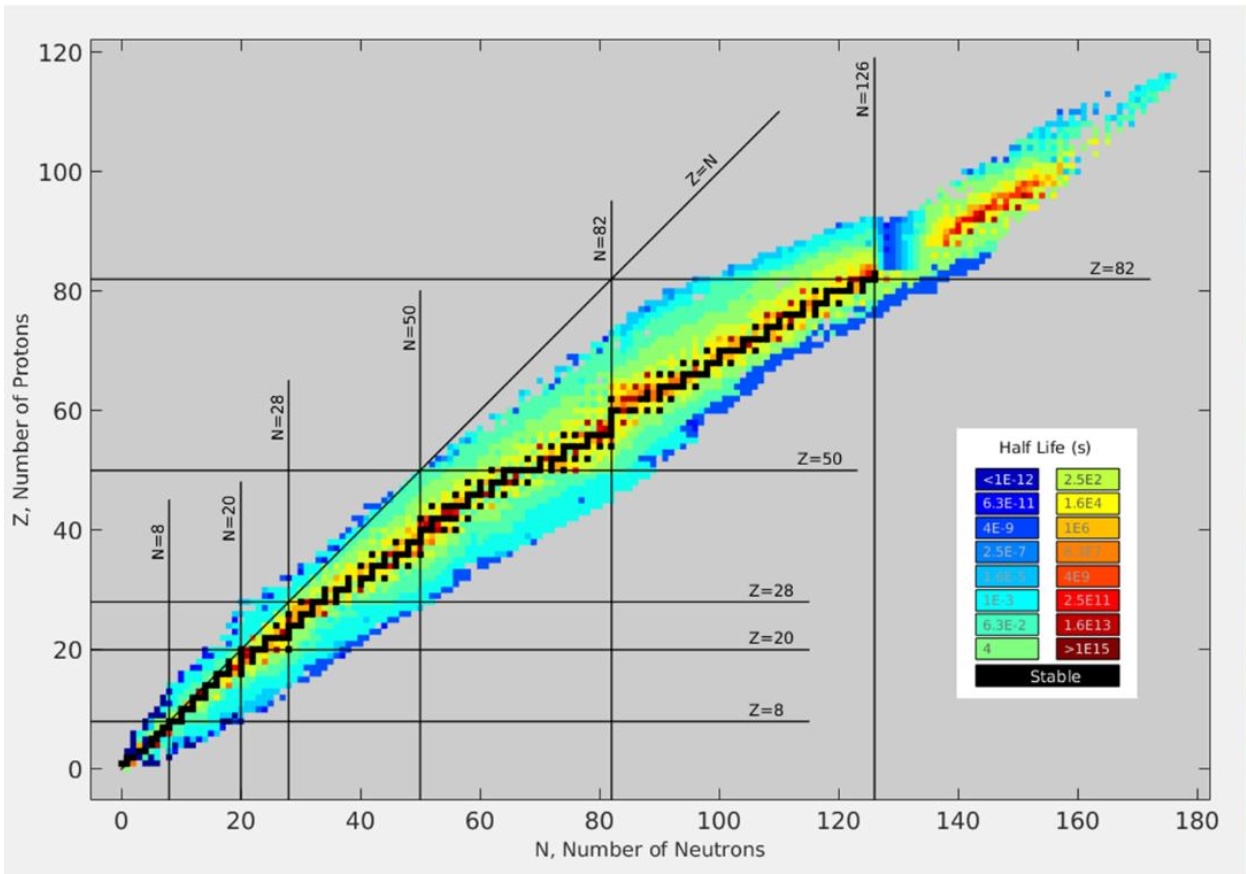
\includegraphics{../figs/nuclides-chart-emilife}
        \caption{Nuclides plotted in $ NZ $ plane as a function of half-life.}
        \label{fig:nuclides-chart-emilife}
    \end{figure}
In figura \ref{fig:nuclides-chart-emilife} sono rappresentati gli stati fondamentali degli oltre 3300 nuclidi a tutt’oggi
noti in funzione di $ N $ e $ Z $ (nelle carte interattive sono rappresentati anche gli stati eccitati o isomeri, 
si veda ad esempio \url{https://www-nds.iaea.org/relnsd/vcharthtml/VChartHTML.html}).
Evidentemente, per ciascun nuclide, in linea orizzontale sono disposti gli isotopi, in linea verticale gli isotoni ed
in linea obliqua gli isobari.
In nero sono indicati i $253$ \emph{nuclidi stabili}, negli altri colori gli oltre $3000$ nuclidi instabili con un
codice colore che da una indicazione del tempo di dimezzamento o emivita
\sidenote{
Secondo la meccanica quantistica i processi fisici sono di natura intrinsecamente statistica per cui è possibile predire
solo la probabilità che avvengano.
Data, pertanto, una popolazione di $ N $ nuclidi la variazione di $ N $ in un tempo elementare $ dt $ sará data dalla
espressione
\[
     dN = - N \lambda dt
\]
dove $ \lambda $ è la \textbf{costante di decadimento del processo} e $ \frac{1}{\lambda} = \tau $ è detta \textbf{vita
    media del processo}. La popolazione in funzione del tempo è allora data da
\[
   N(t) = N(0) e^{- \lambda t}
\]
Spesso, in fisica nucleare ci si riferisce però al \textbf{tempo di dimezzamento} $ t_{1/2} $ definito come il tempo
necessario per dimezzare un qualunque campione di una data sostanza. Si ottiene
\[
 N(t_{1/2}) = N(0) \to t_{1/2} = \frac{\log 2}{\lambda} = \tau \log 2
\]
}. %%TODO Sistemare che esce dal bordo

Un primo fatto rilevante riguarda la distribuzione dei nuclidi nel piano $ ZN $.
Già a colpo d’occhio si apprezza che \textbf{i nuclidi tendono ad avere più neutroni che protoni}.
Si noterà che il quoziente $N/Z$ si scosta sempre più dalla unità con il crescere del numero atomico $A$.
Prendendo come riferimento i nuclidi stabili di ciascuna serie isotopica, si nota che i nuclidi
$ \isotope[4][2]{\mathlarger{He}_{2}} , \isotope[16][8]{\mathlarger{O}_{8}}$ fino a giungere al
$ \isotope[40][20]{\mathlarger{Ca}_{20}} $ giacciono sulla bisettrice con un quoziente $N/Z \sim 1$.
I nuclidi medi come ad esempio $ \isotope[111][48]{\mathlarger{Cd}_{63}} $ hanno un quoziente $N/Z \sim 1.3$.
I nuclidi molto pesanti, infine, come $ \isotope[238][92]{\mathlarger{U}_{146}} $, hanno un quoziente $N/Z \sim 1.6$.


La instabilità nucleare è un fenomeno quantitativamente spettacolare: si va dalla emivita del $ \isotope[6][1]{\mathlarger{H}}
$ di $2.85 \times 10^{-22}$ s a quella del $ \isotope[128][52]{\mathlarger{Te}} $ di $ 2.43 \times 10^{32} $ s ovvero
attraverso $54$ ordini di grandezza!
Man mano che ci si allontana dalla linea dei nuclidi stabili (stability valley) i tempi di dimezzamento si accorciano
progressivamente.
A titolo di esempio si consideri la emivita della serie isotopica dell’indio in figura affianco.

\begin{marginfigure}
    \centering
    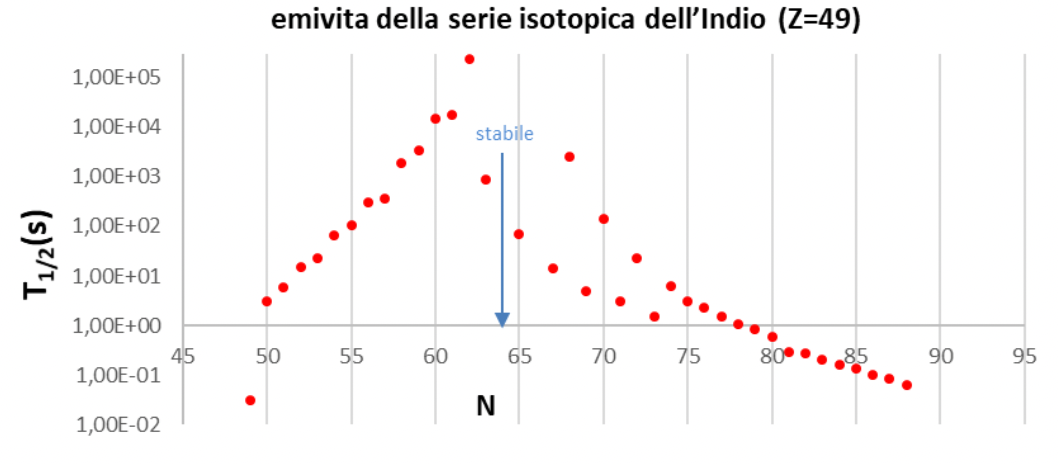
\includegraphics[width = 1.35 \textwidth,scale = 1.5]{../figs/emivita-indio}
%    \caption{Emivita della serie isotopica dell'indio($ Z=49 $)}
    \label{fig:emivita-indio}
\end{marginfigure}

Tornando alla carta dei nuclidi, le linee orizzontali e verticali a $Z$ ed $N = 8, 20, 28, 50, \dots$ detti \textbf{numeri magici},
corrispondono a configurazioni di protoni e neutroni particolarmente stabili (vedi modello a shell)
%%TODO Reference al modello a shell
poiché tali numeri completano le `shell’ nucleari ovvero i livelli energetici più prominenti del potenziale nucleare
medio agente su ciascun protone e neutrone.

Si potrebbe pensare che i nuclidi doppiamente magici siano tutti stabili
ma in realtà non è così.
Certamente si tratta di configurazioni tendenzialmente più stabili delle altre tuttavia non bisogna dimenticare che
la stabilità nucleare è soprattutto legata al corretto quoziente
neutroni/protoni per cui è solo quando \emph{la doppia magicità è compatibile con
un quoziente} $N/Z$ \emph{non troppo lontano} dal necessario che si ha davvero un
nucleo particolarmente stabile.
La dimostrazione di come la doppia magicità tenda a stabilizzare il nuclide è ben visibile nel
$ \isotope[48][20]{\mathlarger{Ca}_{28}} $, stabile nonostante abbia un quoziente $N/Z$ diverso
dai nuclidi della sua regione di numero atomico $A$.

I $253$ nuclidi stabili si estendono lungo una linea a zig-zag nel piano $Z,N$ da $Z=1$ ($ \isotope[1][1]{\mathlarger{H}} $) 
a $Z=83$ ($ \isotope[209][83]{\mathlarger{Bi}} $) quasi senza soluzione di continuità e spesso con
diversi isotopi stabili per ciascun Z. Fanno eccezione $ Tc,Pm(Z=43,Z=61) $ che non hanno alcun nuclide stabile nella
loro serie isotopica.
Al di sopra della serie isotopica del Bismuto i nuclidi sono tutti instabili.

Occorre precisare che i 253 nuclidi stabili sono così suddivisi:
\begin{itemize}
    \item $ 90 $ sono \textbf{teoricamente stabili};
    \item $ 163 $ sono \textbf{osservazionalmente stabili},ovvero teoricamente instabili ma con emivita non misurabile
    con le attuali tecniche.
\end{itemize}

I 253 nuclidi stabili sono stati certamente formati nel Big-bang e nel corso dei processi nucleosintetici all’interno
delle stelle e delle supernovae.
Si hanno inoltre $33$ nuclidi con emivita maggiore di $ {10}^{8}$ anni, stima dell'emivita della Terra, per cui possiamo
affermare che sulla Terra sono osservabili $253+33=286$ \textbf{nuclidi primordiali}.
\begin{figure}
    \centering
    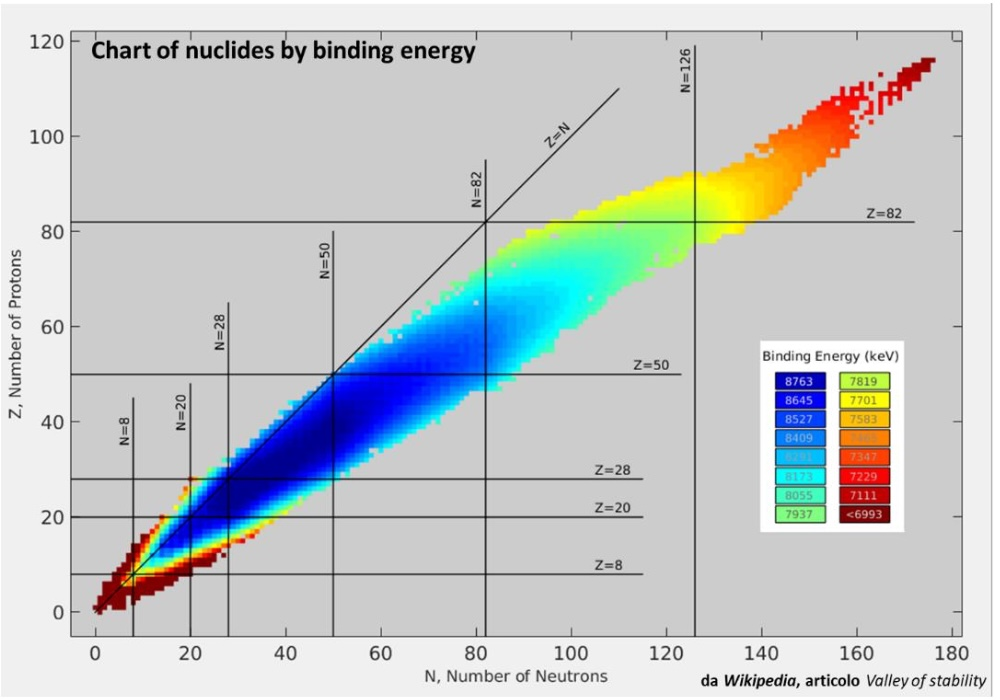
\includegraphics{../figs/nuclides-chart-binding-energy}
    \caption{Chart of nuclides by binding energy.}
    \label{fig:nuclides-chart-binding-energy}
\end{figure}
I $33$ nuclidi instabili primordiali danno origine per decadimento radioattivo ad un certo numero di \emph{nuclidi figli}
spesso di breve o brevissima vita media che certamente non possono essere primordiali.
A questi dobbiamo aggiungere un certo numero di nuclidi generati da \textbf{reazioni nucleari indotte} dai raggi cosmici o dai neutroni naturali.
Di questi ne sono noti $53$ dunque in totale sulla terra sono osservabili $286+53=339$ \textbf{nuclidi naturali}.
I rimanenti, oltre $3000$, sono pertanto \textbf{nuclidi artificiali} prodotti dall’uomo con tecniche differenti.

La carta in figura \ref{fig:nuclides-chart-binding-energy} fornisce informazioni complementari alle precedenti.
Ci attendiamo che, per ciascun valore di Z, l’isotopo stabile sia quello con la maggiore energia di legame per nucleone.
\begin{marginfigure}
    \centering
    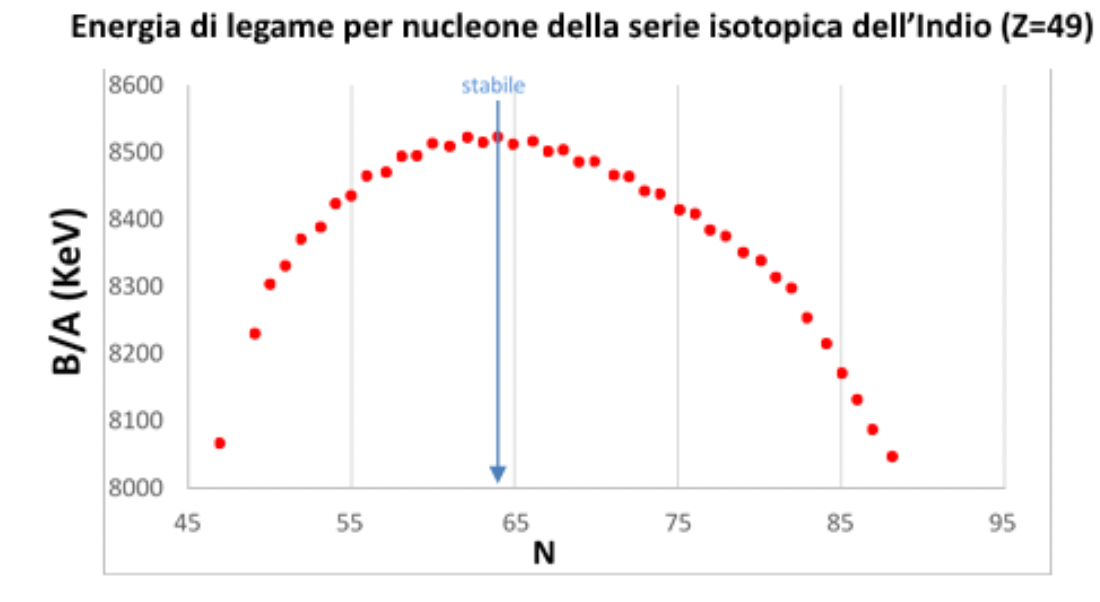
\includegraphics{../figs/indium-binding-energy}
%        \caption{}
    \label{fig:}
\end{marginfigure}
L’andamento di B/A (energia di legame per nucleone) della serie isotopica dell’Indio (Z=49) conferma tale ipotesi.
I valori della energia di legame superano gli 8 MeV per nucleone e sono dell’ordine di 8.5 MeV nel caso dell’isotopo stabile N=64.

Ancora più interessante è \textbf{l’andamento della energia di legame per nucleone dei soli isotopi stabili maggiormente
abbondanti di ciascun nucleo del piano Z, N}. 
Ciò in qualche modo corrisponde alla sezione dell’istogramma bidimensionale della energia di legame lungo la sua linea
mediana corrispondente agli isotopi stabili.
Si ottiene l’andamento seguente:
\begin{figure}
    \centering
    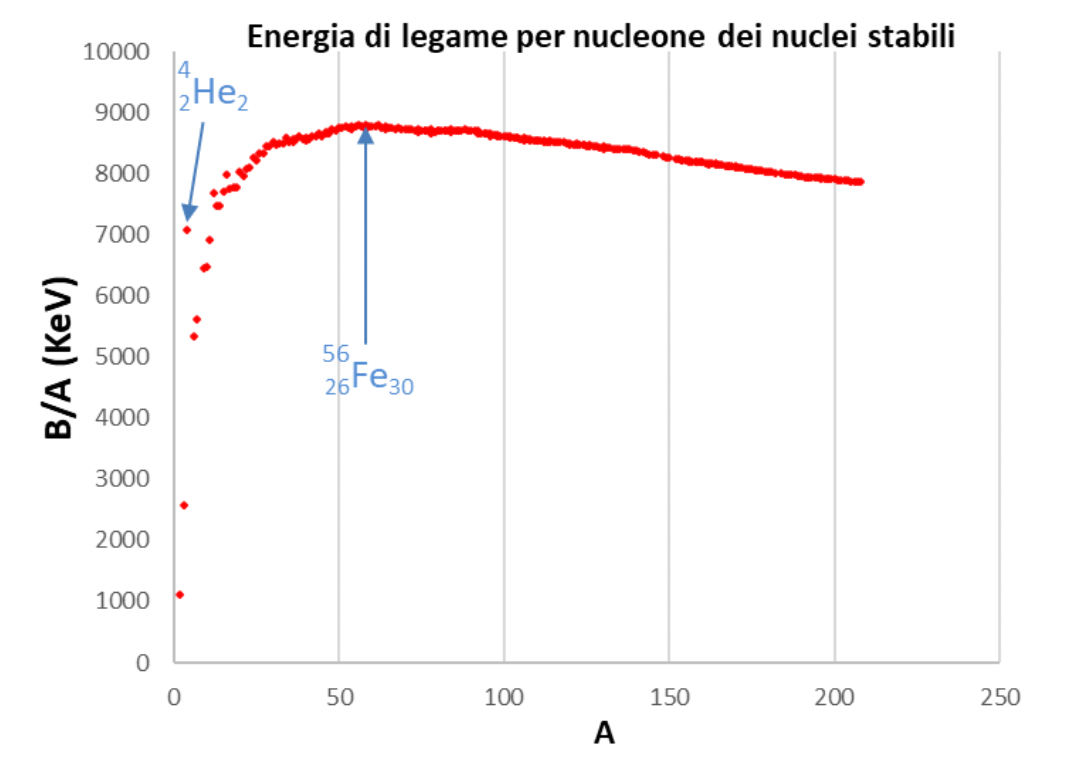
\includegraphics{../figs/binding-energy-stable}
%    \caption{}
    \label{fig:binding-energy-stable}
\end{figure}

Partendo dai nuclei leggeri, il quoziente B/A sale rapidamente raggiungendo un primo picco molto marcato ad oltre 7 MeV
per nucleone nel nucleo di elio da cui risulta che la configurazione nucleare con due protoni e due neutroni è
particolarmente stabile.
Dopo essersi abbassato nel caso del litio (A=6), il quoziente B/A sale con una certa regolarità fino ad un massimo
corrispondente al ferro con 56 nucleoni dove B/A sfiora gli 8.8 MeV per nucleone.
Al di la del ferro il quoziente B/A flette verso il basso con una certa regolarità.
\emph{Uno degli obiettivi dei modelli nucleari è quello di spiegare questo andamento.}
Già nel caso del modello a goccia, il primo ad essere formulato, si ottengono risultati soddisfacenti.

Da ciò che è stato detto al punto precedente segue immediatamente che i nuclei più \emph{leggeri} del ferro guadagnano in
stabilità \emph{aggregando} ulteriori neutroni e protoni mentre i quelli più \emph{pesanti} guadagnano in stabilità 
\emph{perdendo} neutroni e protoni.
Ciò significa che i processi di fusione dei nuclei leggeri e di fissione dei nuclei pesanti saranno esoenergetici
indicando così le due possibili vie per la produzione di energia attraverso reazioni nucleari.
Significa anche che le reazioni nucleari nell’ambito dei processi naturali spontanei (che evolvono sempre verso stati
di maggiore stabilità) tenderanno a fondere i nuclei leggeri e a fissionare quelli pesanti.
La natura ha scelto la fusione dei nuclei leggeri per produrre energia all’interno delle stelle attraverso cicli
successivi che trovano la loro fine nella sintesi del ferro che rende la stella gravitazionalmente instabile fino
determinarne la esplosione.

\begin{figure}
    \centering
    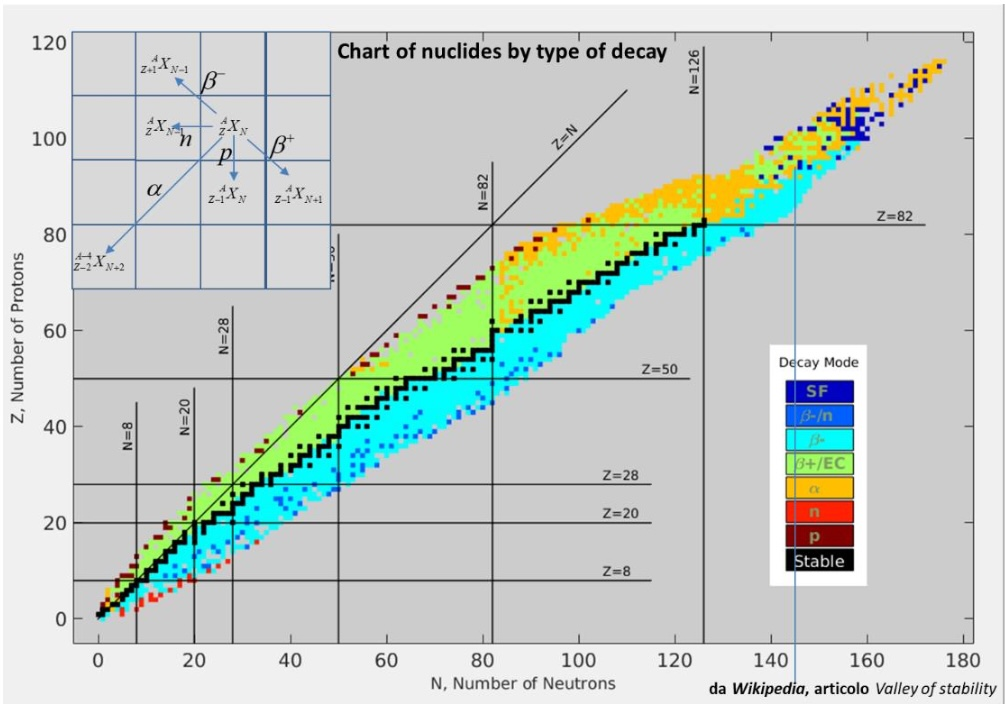
\includegraphics{../figs/nuclides-chart-decay}
    \caption{Chart of nuclides by type of decay.}
    \label{fig:nuclides-chart-decay}
\end{figure}

La carta in figura \ref{fig:nuclides-chart-decay} fornisce una visione d’insieme delle reazioni nucleari cui sono
soggetti i nuclidi instabili.
A colpo d’occhio è evidente che
\begin{itemize}
    \item I nuclidi con un eccesso di neutroni tendono a ristabilire il corretto quoziente N/Z
    attraverso il decadimento $ \beta^-$;
    \item I nuclidi con un eccesso di protoni tendano in generale a ristabilire il corretto quoziente N/Z non attraverso
    il decadimento $ \beta^+$ ma piuttosto attraverso il processo ‘associato’ di cattura elettronica energeticamente più
    vantaggioso $EC$;
    \item I nuclidi pesanti con un forte eccesso di protoni tendono invece a ristabilire il corretto quoziente N/Z
    attraverso il decadimento $ \alpha$.Il decadimento in questione è quello preferenziale per tutti i nuclidi con
    eccesso di protoni al di sopra del piombo (Z=82);
    \item I nuclidi pesantissimi con oltre 100 protoni e 140 neutroni (ad esempio il californio $ \isotope[238][98]{\mathlarger{Cf}_{140}}$)
    sono soggetti a \textbf{fissione spontanea} (SF), ovvero alla frantumazione del nucleo in due nuclei più piccoli seguiti
    da un certo numero di nucleoni liberi perlopiù neutroni;
    \item Alcuni nuclidi leggeri con un forte eccesso di neutroni decadono \textbf{emettendo un neutrone} (n).
    Esempi noti sono alcuni isotopi del boro e del berillio.
\end{itemize}

A titolo di esempio si riportano in figura \ref{fig:decay-chain1} alcune catene di decadimento radioattivo che terminano sugli
isotopi stabili del piombo che vengono raggiunti attraverso una alternanza di decadimenti alfa e beta negativo

\begin{figure}
    \centering
    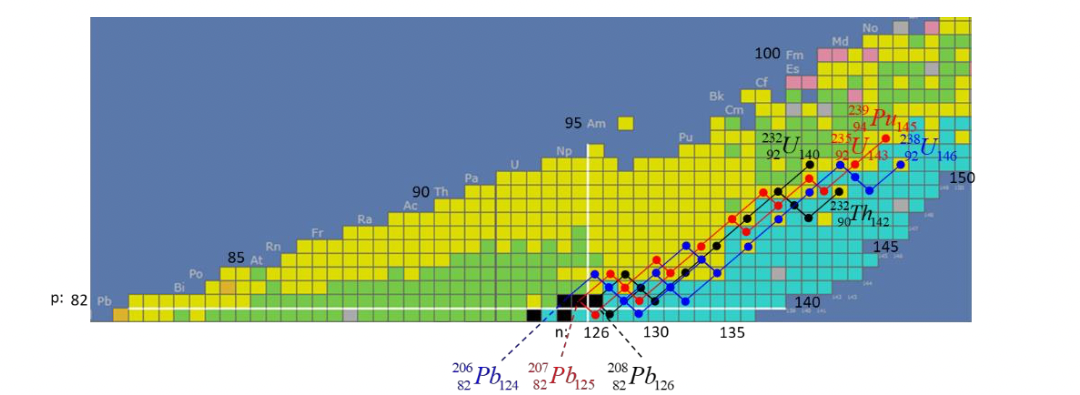
\includegraphics{../figs/decay-chain1}
    \caption{Catene del torio-232/uranio-232 (in nero), dell’uranio-235/plutonio-239 (in rosso) e dell’uranio-238 (blu).}
    \label{fig:decay-chain1}
\end{figure}

Le emivite di ciascun passo della catena possono variare dalla frazione di secondo ai milioni di anni;
l’esempio della catena del torio-232/uranio-232 è reperibile all'indirizzo
\url{https://en.wikipedia.org/wiki/Decay_chain#/media/File:Decay_Chain_Thorium.svg}.